\documentclass[11pt]{article}
\usepackage[a4paper, portrait, margin=1in]{geometry}
\usepackage{hyperref}
\usepackage{graphicx}
\usepackage{fancyhdr}
\usepackage{verbatim}
\usepackage[labelfont=bf]{caption}
\usepackage{color}
\usepackage{hyperref}
\usepackage{footnotebackref}
\usepackage{amsthm}
\usepackage{multirow}
\usepackage{nicefrac}

\pagestyle{fancy}
\fancyhf{}
\renewcommand{\headrulewidth}{0pt}
\renewcommand{\footrulewidth}{0pt}

\fancypagestyle{firstpagefooter}
{
\lfoot{Version: 29.09.2016}
\cfoot{}
\rfoot{\thepage}
}
\cfoot{\thepage}

\hypersetup
{
    colorlinks=true,
    linkcolor=blue,
    citecolor=blue,
    filecolor=blue,
    urlcolor=blue,
    linktoc=page            % Link only on page number
}

\renewcommand{\qedsymbol}{}
\newtheorem{hyp}{Hypothesis}
\theoremstyle{definition}
%\newtheorem*{ana}{Analysis}
\newenvironment{ana}[1][\proofname]{\begin{proof}[Analysis]}{\end{proof}}

% Timestamps (DO NOT CHANGE!)
\newcommand\Tarr{T_{\mathrm{arr}}}
\newcommand\Tenq{T_{\mathrm{enq}}}
\newcommand\Tdeq{T_{\mathrm{deq}}}
\newcommand\Tsent{T_{\mathrm{sent}}}
\newcommand\Trecv{T_{\mathrm{recv}}}
\newcommand\Tleft{T_{\mathrm{left}}}

% Macros.
\renewcommand\b[1]{{\bf{#1}}}
\newcommand\p{^\prime}
\renewcommand\t\texttt
\newcommand\md[2]{\left[#1\mathrm{\ mod\ }#2\right]}
\newcommand\td{{\color{red}\b{\textsf{[TODO]}}}}
\newcommand\plotscale{1.2}
\newcommand\baselined{01\char`_memcached\char`_baselines\char`_16-10-21\char`_08:20:35}
\newcommand\baseline{01_memcached_baselines_16-10-21_08:20:35}
\newcommand\traced{02\char`_stability\char`_trace\char`_16-10-20\char`_20:38:14}
\newcommand\trace{02_stability_trace_16-10-20_20:38:14}

\begin{document}

\title{Advanced Systems Lab (Fall'16) -- First
Milestone}

\author{\textbf{Name: \emph{Fabio M. Banfi}}\\\textbf{Legi number: \emph{09-917-972}}}

\date{
\vspace{4cm}
\textbf{Grading} \\
\begin{tabular}{|c|c|}
\hline  \textbf{Section} & \textbf{Points} \\
\hline  1.1 &  \\ 
\hline  1.2 &  \\ 
\hline  1.3 &  \\ 
\hline  1.4 &  \\ 
\hline  2.1 &  \\ 
\hline  2.2 &  \\ 
\hline  3.1 &  \\ 
\hline  3.2 &  \\ 
\hline  3.3 &  \\ 
\hline \hline Total & \\
\hline 
\end{tabular} 
}

\maketitle
\thispagestyle{firstpagefooter}

\clearpage
%%%%%%%%%%%%%%%%%%%%%%%%%%%%%%%%%%%%%%%%%%%%%%%%%%%%%%%%%%%%%%%%%%%%%%%%%%%%%%%%%%%%%%%%%%%%%%%%%%%
%%%%%%%%%%%%%%%%%%%%%%%%%%%%%%%%%%%%%%%%%%%%%%%%%%%%%%%%%%%%%%%%%%%%%%%%%%%%%%%%%%%%%%%%%%%%%%%%%%%
\section{System Description}\label{sec:system-description}
%%%%%%%%%%%%%%%%%%%%%%%%%%%%%%%%%%%%%%%%%%%%%%%%%%%%%%%%%%%%%%%%%%%%%%%%%%%%%%%%%%%%%%%%%%%%%%%%%%%
%%%%%%%%%%%%%%%%%%%%%%%%%%%%%%%%%%%%%%%%%%%%%%%%%%%%%%%%%%%%%%%%%%%%%%%%%%%%%%%%%%%%%%%%%%%%%%%%%%%

%%%%%%%%%%%%%%%%%%%%%%%%%%%%%%%%%%%%%%%%%%%%%%%%%%%%%%%%%%%%%%%%%%%%%%%%%%%%%%%%%%%%%%%%%%%%%%%%%%%
\subsection{Overall Architecture}\label{sec:desc:architecture}
%%%%%%%%%%%%%%%%%%%%%%%%%%%%%%%%%%%%%%%%%%%%%%%%%%%%%%%%%%%%%%%%%%%%%%%%%%%%%%%%%%%%%%%%%%%%%%%%%%%

\begin{comment}
The system implements a \emph{key-value store} and consists of three components: a set of \emph{servers}, a set of \emph{clients}, and a \emph{middleware}.
The set of servers is instantiated by a set of (virtual) machines running \t{memcached}\footnote{\url{https://memcached.org/}}.
Thus each server alone coincides with a key-value store, but in this system the clients see the middleware as a single key-value store.
The set of clients is instantiated by a set of (virtual) machines running \t{memaslap}\footnote{\url{http://docs.libmemcached.org/bin/memaslap.html}} from the \t{limmemcached} library, which generates fully synthetic workloads for \t{memcached}.
At the heart of the system, the middleware acts as a \emph{load balancer} for client's requests to the servers.
%Note that therefore the number of servers is not necessarily known to the clients.
\end{comment}

The middleware has been implemented in Java 7, following the provided guideline as shown in Figure~\ref{fig:middleware}.
The diagram also shows the structure of the program in terms of objects when the middleware is connected to three clients and three servers.
The objects are boxed in blue, and the instance names are used as labels.
Embracing a minimal design philosophy, the program consists of just five classes (not counting the provided interface \t{RunMW}), of which only three \emph{core} classes contribute the actual logic of the middleware.
Those are \t{Middleware}\footnote{\mbox{\url{https://gitlab.inf.ethz.ch/fbanfi/asl-fall16-project/blob/master/src/middleware/Middleware.java}}}, \t{ServerWriter}\footnote{\mbox{\url{https://gitlab.inf.ethz.ch/fbanfi/asl-fall16-project/blob/master/src/middleware/ServerWriter.java}}}, and \t{ServerReader}\footnote{\mbox{\url{https://gitlab.inf.ethz.ch/fbanfi/asl-fall16-project/blob/master/src/middleware/ServerReader.java}}}.

\t{Middleware} is responsible for starting the middleware itself and also for accepting, reading, and addressing clients' requests (by \emph{load balancing}).
This is all handled by the function \t{Middleware.run()}, which is documented in more detail in Section~\ref{sec:desc:hashing}.
As Figure~\ref{fig:middleware} shows, \t{Middleware} has members \t{serverWriter}, an array of \t{ServerWriter} instances, and \t{serverReader}, an array of \t{ServerReader} instances.

\t{ServerWriter} handles all the \t{SET} requests generated by the clients, as well as \t{DELETE} requests (even though %the latter
those are \emph{not} generated by \t{memaslap}).
On the other hand, \t{ServerReader} handles all the \t{GET} requests. % generated by the clients.
Both classes possess an internal queue where the requests to be processed have to be written. % (by \t{Middleware.run()}).
More detailed description of those two classes are given in Section~\ref{sec:desc:writes} and Section~\ref{sec:desc:reads}, respectively.

The other two classes are \t{Request}\footnote{\mbox{\url{https://gitlab.inf.ethz.ch/fbanfi/asl-fall16-project/blob/master/src/middleware/Request.java})}} and \t{Helper}\footnote{\mbox{\url{https://gitlab.inf.ethz.ch/fbanfi/asl-fall16-project/blob/master/src/middleware/Helper.java}}}.
\t{Helper} contains constant values (such as buffer sizes), some useful functions and structures used by the core classes, as well as some functions for testing and debugging.
Finally, \t{Request} instances encapsulate client requests along with the associated client connections (as sockets), as well as timing information.
The latter consist of six timestamps, $\Tarr$, $\Tleft$, $\Tenq$, $\Tdeq$, $\Tsent$, and $\Trecv$.
The code has been instrumented to take those timestamps for each request as depicted in Figure~\ref{fig:middleware}.
Note that the responses of the servers are given back to the clients by \t{ServerWriter} and \t{ServerReader} instances, contrary to what the diagram may suggest.
More details on when exactly such timestamps are taken follow in the next sections.

\begin{figure}[h]
    \centering
    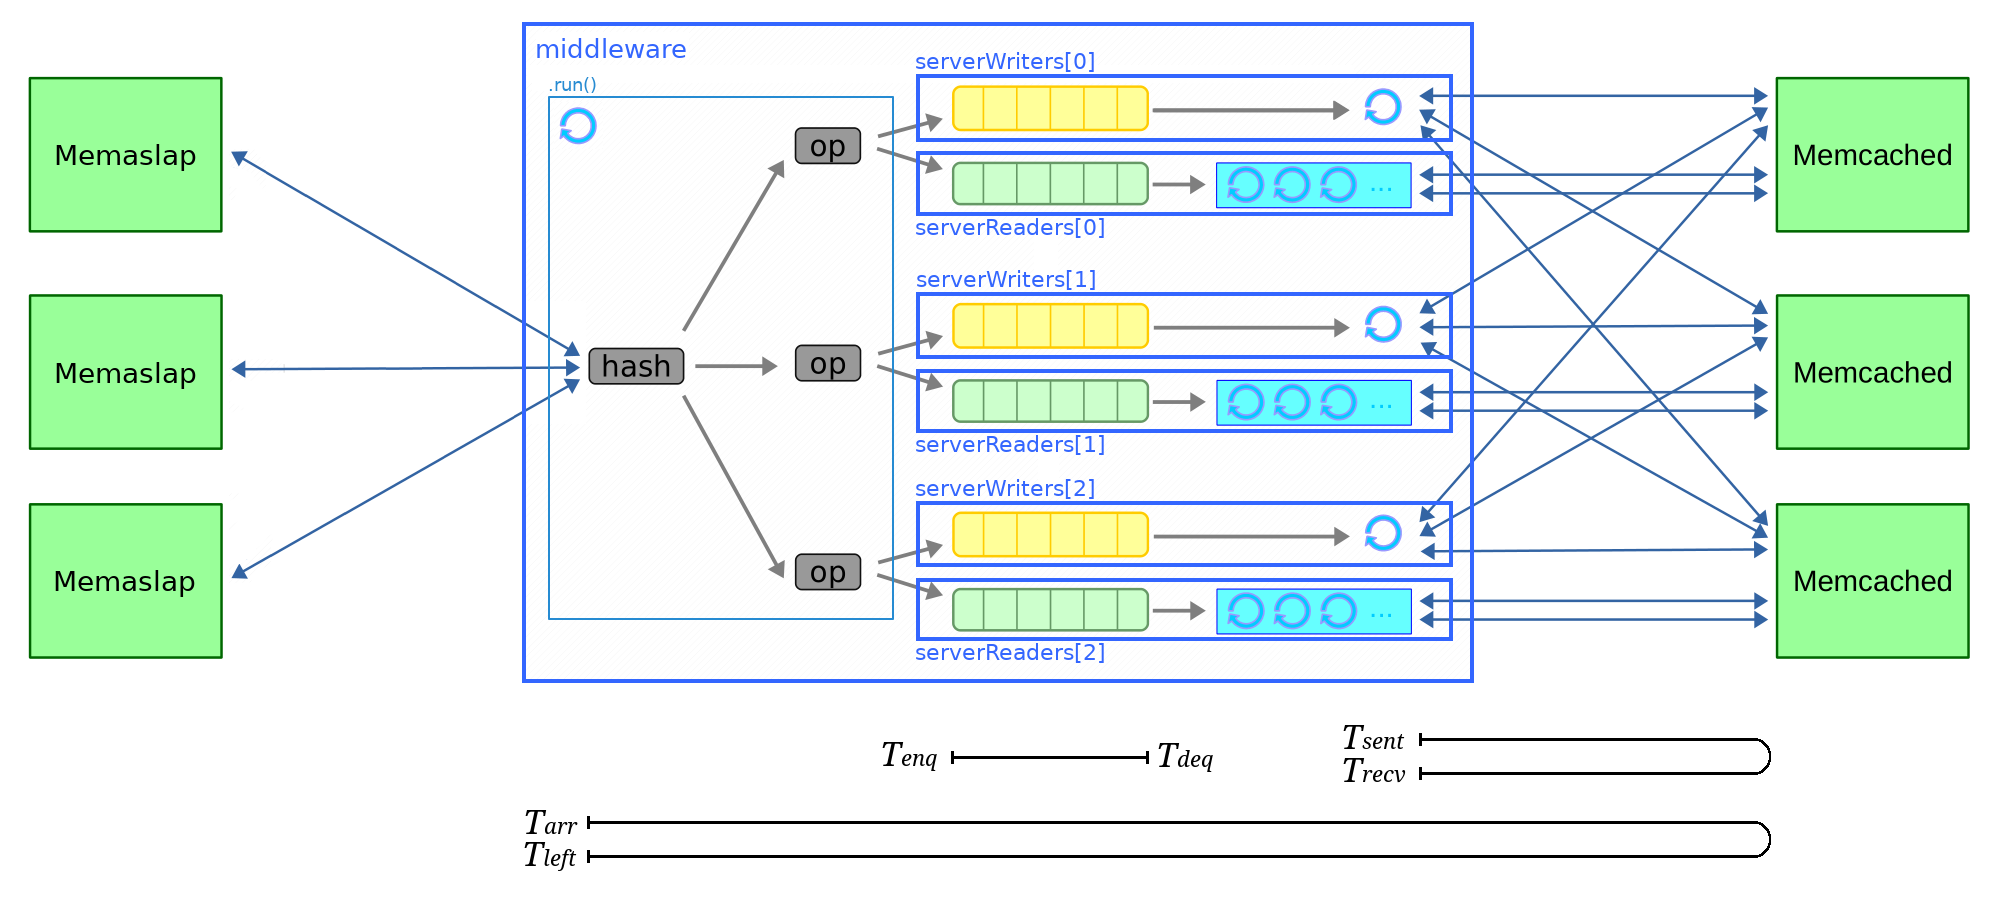
\includegraphics[scale=0.22]{imgs/middleware}
    \caption{Middleware architecture diagram.}
    \label{fig:middleware}
\end{figure}

%%%%%%%%%%%%%%%%%%%%%%%%%%%%%%%%%%%%%%%%%%%%%%%%%%%%%%%%%%%%%%%%%%%%%%%%%%%%%%%%%%%%%%%%%%%%%%%%%%%
\subsection{Load Balancing and Hashing}\label{sec:desc:hashing}
%%%%%%%%%%%%%%%%%%%%%%%%%%%%%%%%%%%%%%%%%%%%%%%%%%%%%%%%%%%%%%%%%%%%%%%%%%%%%%%%%%%%%%%%%%%%%%%%%%%

The function \t{Middleware.run()} \emph{asynchronously} accepts connections from \t{memaslap} clients by means of \t{java.nio}'s selectors and channels.
Each connected client's request is read at once into a buffer, and the byte-sequences corresponding to the operation (\t{SET}, \t{GET}, or \t{DELETE}) and the key (assumed to consist of exactly 16 bytes) are extracted.
\emph{Load balancing} is implemented by first hashing the key into a value from $0$ to $N-1$ (where $N$ is the number of servers), and then using the obtained integer as an index to select the appropriate \t{ServerWriter}/\t{ServerReader} instance (depending by the operation) to which forward the request.

The hashing of the keys is implemented by first converting the sequence of 16 bytes into a string, then calling \t{String.hashCode()} on the latter, and finally computing the reminder of the obtained number when divided by $N$.
For strings, Java's \t{hashCode()} uses a product sum algorithm over the entire text\footnote{\url{http://bugs.java.com/bugdatabase/view_bug.do?bug_id=4045622}}.
Therefore, combining those steps and assuming that the key consists of the byte sequence $K=k_0,k_1,\ldots,k_{15}$, the obtained hash value is the integer\footnote{The notation $\md kn$ represents the remainder of $k$ divided by $n$.}
\[h_N(K)\doteq\md{\sum_{i=0}^{15}k_i\cdot31^{15-i}}N\in\{0,\ldots,N-1\}.\]

Since the middleware must act as a load balancer, it is important that it distributes the requests uniformly among the $N$ servers.
Assuming a source of uniform random sequences of 16 bytes (where each possible sequence of 16 bytes is picked with the same probability, or equivalently, each number in the interval $\{0,\ldots,2^{128}-1\}$ is equiprobable), one would expect that the hash function $h_N$ defined above, when attached to such a source, acts itself as a source of uniform random integers in the interval $\{0,\ldots,N-1\}$.
More formally, we require $h_N(\b U_{2^{128}})=\b U_N$, where $\b U_n$ is defined as the uniform random variable over $\{0,\ldots,n-1\}$.

As a formal proof of this fact would be out of scope, an heuristic argument has been used to justify the choice of $h_N$.
Let define the \emph{statistical distance} between two probability distributions $\b P$ and $\b Q$ over a finite set $\mathcal X$ as the \emph{total variation distance}, that is, the $1$-norm of the difference of the two probability distributions, formally
\[\delta(\b P,\b Q)\doteq\frac12\sum_{x\in\mathcal X}\left\vert\b P(x)-\b Q(x)\right\vert.\]
Thus, letting $\b H_N\doteq h_N(\b U_{2^{128}})$, we wish for $\delta(\b H_N,\b U_N)$ to be \emph{as close as possible to zero}.
For $N=2,\ldots,7$, the function \t{Helper.testHashFunction()} prints the statistical distance as defined above between the uniform distribution and an empirical version $\widetilde\b H_N$ of the distribution $\b H_N$.
%The output of the hash function $h_N$ on input (pseudo-)random $16$ bytes sequences.
Concretely, for each value of $N$, 10'000'000 pseudo-random $16$ bytes sequences were fed to $h_N$, and the output was used to fill the corresponding of $N$ buckets (each one representing a server).
The empirical distribution $\widetilde\b H_N=h_N(\widetilde\b U_{2^{128}})$ was then drawn from those buckets, where the pseudo-random source $\widetilde\b U_{2^{128}}$ has been instantiated by \t{new BigInteger(128, new Random())}.
The results of a run of this experiment are shown in Table~\ref{tab:hash}, which clearly shows that $\widetilde\b H_N$ is very close to the uniform distribution $\b U_N$ for all used values of $N$, exactly as desired.

\begin{table}[h]
    \centering
    \small
    {
        \smallskip
        \begin{tabular}{|c|c||c|c|}
            \hline
            $N$ & $\delta(\widetilde\b H_N,\b U_N)$ & $N$ & $\delta(\widetilde\b H_N,\b U_N)$ \\
            \hline
            \hline
            $2$ & $0.000236$ & $5$ & $0.000292$ \\ 
            $3$ & $0.000321$ & $6$ & $0.000239$ \\  
            $4$ & $0.000262$ & $7$ & $0.000221$ \\ 
            \hline 
        \end{tabular}
    }
    \caption{Results of the statistical distance test on the chosen hash function.}
    \label{tab:hash}
\end{table}

%%%%%%%%%%%%%%%%%%%%%%%%%%%%%%%%%%%%%%%%%%%%%%%%%%%%%%%%%%%%%%%%%%%%%%%%%%%%%%%%%%%%%%%%%%%%%%%%%%%
\subsection{Write Operations and Replication}\label{sec:desc:writes}
%%%%%%%%%%%%%%%%%%%%%%%%%%%%%%%%%%%%%%%%%%%%%%%%%%%%%%%%%%%%%%%%%%%%%%%%%%%%%%%%%%%%%%%%%%%%%%%%%%%

An instance of \t{ServerWriter} handles all the \t{SET} and \t{DELETE} requests associated with a specific \emph{primary} server.
Since it is possible to define a replication factor $R$ when starting the middleware, each instance of the array \t{Middleware.serverWriters} opens $R$ parallel connections with $R$ different servers, where $R-1$ of them are \emph{secondary}.
Assuming that \t{serverWriters[$i$]} is associated with primary server $1\leq i\leq N$, then it opens connections with the servers
\[i,\md{i+1}N,\ldots,\md{i+R-1}N.\]

\t{serverWriters[$i$]} has member \t{queue} of type \t{LinkedBlockingQueue<Request>}, which is \emph{thread-safe}.
The method \t{serverWriters[$i$].enqueue(Request)} allows to safely put a new request (whose key's hash is $i$) into this queue.
The timestamp $\Tenq$ is taken just \emph{before} this function call.

\t{serverWriters[$i$]} also defines a thread class \t{ServerWriter.WriterThread}, of which it starts a \emph{single} instance.
The method \t{ServerWriter.WriterThread.run()} is where all the write logic takes place.
\begin{comment}
Asynchronous networking is implemented as follows:
\begin{enumerate}
    \item Send a request.
    \item If no response is available, goto 1.
    \item Process responses.
\end{enumerate}
Therefore, \t{run()} consists of an infinite loop
\end{comment}
The communications with the replication servers happen asynchronously.
%, and thus \t{run()} consists of an infinite loop%
%, where a
At the beginning, the top request on the queue \t{queue}, if any, is safely removed.
This is accomplished by calling the semi-blocking function \t{queue.poll(10, TimeUnit.MILLISECONDS)}.
Note that the second parameter indicates a $10\ ms$ timeout\footnote{The timeout has been used to avoid that the middleware consumes 100\% of the CPU time when there are no clients requests. It has been observed that the throughput is positively affected by this, since it is higher compared to when there is no timeout.} %, and also because it has been observed that the throughput is positively affected by introducing a small ``sleeping time''.}
after which, if no elements was removed from the queue% (because it remained empty for that time interval)
, the function call stops to block.
If a request to be processed was successfully removed from \t{queue}, that is, the call to \t{poll} returned something other than \t{null}, then the timestamp $\Tdeq$ is taken and the request is forwarded to the $R$ servers.
This is done in a sequential fashion, that is, the request is first sent to server $i$, then to server $\md{i+1}N$, and so on until it is finally sent to server $\md{i+R-1}N$.
The timestamp $\Tsent$ is taken right \emph{after} sending the request to the primary server $i$.

After polling the queue for new requests, \t{run()} checks whether there are responses from the servers ready to be read.
If this is the case, all the available responses are processed one after the other.
Once the responses are all processed (and hence only when there were responses to process in the first place), \t{run()} checks which responses it can forward back to which client\footnote{This is accomplished by keeping a queue of sent requests, but for which a response has not yet been received, as well as a queue for each server which holds all its responses which have not yet been forwarded to the clients. Once \emph{all} the response queues are non-empty, it means that a response is ready for the request at the top of the sent requests queue. Assuming that \t{memcached} keeps responses ordered in time, the response to this request corresponds exactly to all the top elements of the servers' queues.}.
For this, the policy is that a response is sent back to the client which originated the corresponding request only once \emph{all} the replications servers gave their response.
Moreover, in case of a \t{SET} request, the response \t{STORED} is sent back to the client only if \emph{all} the responses from the servers were \t{STORED}, and otherwise the response \t{ERROR} is sent to the client.
The same applies to \t{DELETE} requests, where \t{STORED} is replaced by \t{DELETED}, and \t{ERROR} by \t{NOT\char`_FOUND}.
The timestamp $\Trecv$ is defined to be the \emph{maximum} between the times at which each server gave its response, which for each server is taken right \emph{after} receiving the answer.
Finally, the timestamp $\Tleft$ is taken right \emph{after} the response has been sent to the clients.
After logging the timing information of the request, the thread starts this process afresh by calling again \t{queue.poll(10, TimeUnit.MILLISECONDS)}.

A quick inspection of the three clients log files from \hyperref[f:trace]{\t{trace}} reveals that write operations take about one and a half of the time needed for read operations (about $15\,000\ \mu s$ vs. $10\,000\ \mu s$ for total average response time).
\begin{hyp}
    The rate at which writes can be carried out in the system is likely to be limited by either the specified number of replication servers, the sequential sending to the replication servers, the saturation of \t{memcached}'s database, or a combination of those factors.
\end{hyp}

\begin{comment}
\begin{ana}
    Deferred to later milestones.
\end{ana}
\end{comment}

\clearpage
%%%%%%%%%%%%%%%%%%%%%%%%%%%%%%%%%%%%%%%%%%%%%%%%%%%%%%%%%%%%%%%%%%%%%%%%%%%%%%%%%%%%%%%%%%%%%%%%%%%
\subsection{Read Operations and Thread Pool}\label{sec:desc:reads}
%%%%%%%%%%%%%%%%%%%%%%%%%%%%%%%%%%%%%%%%%%%%%%%%%%%%%%%%%%%%%%%%%%%%%%%%%%%%%%%%%%%%%%%%%%%%%%%%%%%

An instance of \t{ServerReader} handles all the \t{GET} requests associated with a specific server.
Even though it is possible to define a replication factor $R$ when starting the middleware, each instance of \t{Middleware.serverReaders} only accesses the value on the primary server, ignoring the content of the secondary servers (if any) for the specific key.

For any $1\leq i\leq N$, \t{serverReaders[$i$]} starts a \emph{thread pool} of size $T$, as specified when starting the middleware.
The threads in the pool are all instances of \t{ServerReader.ReaderThread}, and each first opens its own separate connection with the primary server $i$.
\t{serverReaders[$i$]} also defines a queue \t{queue} for incoming requests to be forwarded to the associated server.
Since potentially more than one thread can read from the queue \t{serverReaders[$i$].queue}, the latter has to be \emph{thread-safe}, and thus it has been instantiated as a \t{LinkedBlockingQueue<Request>}.
The method \t{serverReaders[$i$].enqueue(Request)} allows to safely put a new request (whose key's hash is $i$) into this queue, and internally it just calls \t{queue.put(Response)}. % to safely add a request to the queue.
The timestamp $\Tenq$ is taken right \emph{before} this function call.

Being synchronous, the reading logic is very simple.
It takes place inside the function \t{ServerReader.ReaderThread.run()}.
First, the thread extracts an element from the queue by calling \t{queue.take()}, which blocks until an element was successfully removed from the queue (and thus in particular blocks the thread as long as the queue is empty).
The timestamp $\Tdeq$ is taken right \emph{after} this function call.
Subsequently, once an element has been successfully extracted, the thread sends it to the server and waits (blocking) until the server produces an answer.
The timestamps $\Tsent$ and $\Trecv$ are taken right \emph{after} sending the request to the server right \emph{after} receiving an answer, respectively.
Finally the thread forwards the response to the client that originated the request, and takes the timestamp $\Tleft$ right \emph{afterwards}.
After logging the timing information of the request, the thread starts this process afresh by calling again \t{queue.take()}.

%%%%%%%%%%%%%%%%%%%%%%%%%%%%%%%%%%%%%%%%%%%%%%%%%%%%%%%%%%%%%%%%%%%%%%%%%%%%%%%%%%%%%%%%%%%%%%%%%%%
%%%%%%%%%%%%%%%%%%%%%%%%%%%%%%%%%%%%%%%%%%%%%%%%%%%%%%%%%%%%%%%%%%%%%%%%%%%%%%%%%%%%%%%%%%%%%%%%%%%
\section{Memcached Baselines}\label{sec:baseline}
%%%%%%%%%%%%%%%%%%%%%%%%%%%%%%%%%%%%%%%%%%%%%%%%%%%%%%%%%%%%%%%%%%%%%%%%%%%%%%%%%%%%%%%%%%%%%%%%%%%
%%%%%%%%%%%%%%%%%%%%%%%%%%%%%%%%%%%%%%%%%%%%%%%%%%%%%%%%%%%%%%%%%%%%%%%%%%%%%%%%%%%%%%%%%%%%%%%%%%%

The memcached baseline experiment aims at analyzing the behavior of \t{memcached} without the presence of the middleware.
The experiment setup is outlined in Table~\ref{tab:exp1}.

\begin{table}[!h]
    \centering
    \small
    {
        \smallskip
        \begin{tabular}{|c|c|}
            \hline \b{Servers} & 1 $\times$ A2 \\ 
            {Threads / machine} & 1 \\ 
            \hline\hline \b{Clients} & 2 $\times$ A2 \\ 
            Virtual clients / machine & 2 to 64, step 2 \\ 
            {Keys size} & 16B \\
            {Values size} & 128B \\
            {Writes} & 1\% \\
            {Overwrite proportion} & 90\% \\
            \hline\hline \b{Middleware} & Not present \\ 
            \hline\hline Runtime $\times$ repetitions & 30s $\times$ 5 \\ 
            Log files & \hyperref[f:baseline]{\t{baseline}} \\
            \hline 
        \end{tabular}
    }
    \caption{Memcached baselines experiment setup.}
    \label{tab:exp1}
\end{table}

\begin{comment}
For this, %as reported in Table~\ref{tab:exp1}, 
a single server machine running \t{memcached} (type A2) and two client machines running \t{memaslap} (type A2) have been used from the provided machines on Microsoft Azure.
All the three machines have been run in parallel for 16 rounds.
At round $i$, the server (re)starts \t{memcached} on one thread (\t{-t 1}) and both clients start a single \t{memaslap} instance for 30 seconds (\t{-t 30s}) with $4i$ virtual clients (\t{-T $4i$ -c $4i$}) and overwrite ratio 0.9 (\t{-o 0.9}).
%Therefore, the server receives request from 8 virtual clients at the first round, 16 at the second, 24 at the third and so on until it receives requests from a total of 128 virtual clients at the last step.
The configuration file used by both clients is located at
\url{https://gitlab.inf.ethz.ch/fbanfi/asl-fall16-project/blob/master/config/smallvalue.cfg}, and it specifies a workload of 16B keys and 128B values, as well as a 1\% proportion of writes.
Finally, \t{memaslap} has been set to collect statistics every second (\t{-S 1}).

The extracted data are \emph{throughput} (\hyperref[f:tps1]{TPS1}) and \emph{response time} (as mean value and standard deviation, \hyperref[f:rt1]{RT1}).
In order to get more precise data, each round consists of 5 repetitions, where the average of each of the three data %(throughput, mean and standard deviation of response time) 
has been taken.
Then for each step, the resulting throughput of the two clients has been added up, while for both mean and standard deviation the average has been taken.
\end{comment}

The experiment is carried out completely by the script located at \url{https://gitlab.inf.ethz.ch/fbanfi/asl-fall16-project/blob/master/scripts/experiments/01_memcached_baselines}, which collects \emph{all} the \t{memaslap} outputs (\t{*.log}, inclusive repetitions), all the extracted data (\t{tps.data} for the throughput and \t{rt.data} for the response time), and also produces plots of the latter.
Note that the throughput measured at each second by the two \t{memaslap} clients have been added up, while mean and standard deviation of the response times have been averaged.
The throughput is depicted in Figure~\ref{fig:baseline_tps_cloud}, and the response time in Figure~\ref{fig:baseline_rt_cloud}.

%%%%%%%%%%%%%%%%%%%%%%%%%%%%%%%%%%%%%%%%%%%%%%%%%%%%%%%%%%%%%%%%%%%%%%%%%%%%%%%%%%%%%%%%%%%%%%%%%%%
\subsection{Throughput}\label{sec:baseline:tput}
%%%%%%%%%%%%%%%%%%%%%%%%%%%%%%%%%%%%%%%%%%%%%%%%%%%%%%%%%%%%%%%%%%%%%%%%%%%%%%%%%%%%%%%%%%%%%%%%%%%

\begin{hyp}
    The throughput as a function of connected clients should initially grow quasi-linearly, an then reach a saturation point at which no more growth is observed.
    Eventually, when the number of clients becomes too large, the throughput may even start to decrease.
\end{hyp}

\begin{ana}
    Figure~\ref{fig:baseline_tps_cloud} confirms in part this hypothesis.
    The quasi-linear growth is observed from 2 to about 16 clients.
    There seems to be a saddle point around 20 clients, but this is probably an artifact caused by the latencies of the connections.
    Then the throughput continues to grow, but at a much slower rate, which indicates that a saturation point has been hit, or is soon to be hit.
    Starting from 96 clients an even lower increase is observed, strengthening the possibility of having a saturation point at about 100.
    Nevertheless, the number of clients is too low so see an effective saturation, or even a degradation of the throughput.
\end{ana}

\begin{comment}
\begin{figure}[!h]
    \centering
    \includegraphics[scale=1]{../../log/experiments/LOCAL_01_memcached_baselines_16-10-18_11:01:45/tps.pdf}
    \caption{Throughput of middleware connected to 3 clients and 3 servers with full replication on local machine.}
    \label{fig:baseline_tps_local}
\end{figure}
\end{comment}

\begin{figure}[!h]
    \centering
    \includegraphics[scale=\plotscale]{../../log/experiments/\baseline/tps.pdf}
    \caption{Throughput by baseline experiment.}
    \label{fig:baseline_tps_cloud}
\end{figure}

%%%%%%%%%%%%%%%%%%%%%%%%%%%%%%%%%%%%%%%%%%%%%%%%%%%%%%%%%%%%%%%%%%%%%%%%%%%%%%%%%%%%%%%%%%%%%%%%%%%
\subsection{Response time}\label{sec:baseline:rt}
%%%%%%%%%%%%%%%%%%%%%%%%%%%%%%%%%%%%%%%%%%%%%%%%%%%%%%%%%%%%%%%%%%%%%%%%%%%%%%%%%%%%%%%%%%%%%%%%%%%

\begin{hyp}
    The average response time in function of the number of connected clients should grow constantly for a short period of time, and then it should hit a saturation point where it should start to grow linearly.
    It may eventually hit a point where the grow rate increases even more.
\end{hyp}

\begin{ana}
    From Figure~\ref{fig:baseline_tps_cloud}, it results that the average response time is almost constant for up to 10 clients, but then clearly starts to grow linearly until 128.
    Nevertheless, a point where the grow rate increases even more is not observed.
    Figure~\ref{fig:baseline_tps_cloud} also shows the standard deviation of the response time.
    It results that this grows linearly as well.
\end{ana}

\clearpage

\begin{comment}
\begin{figure}[!h]
    \centering
    \includegraphics[scale=1]{../../log/experiments/LOCAL_01_memcached_baselines_16-10-18_11:01:45/rt.pdf}
    \caption{Average and standard deviation of response time of middleware connected to 3 clients and 3 servers with full replication on local machine.}
    \label{fig:baseline_rt_local}
\end{figure}
\end{comment}

\begin{figure}[!h]
    \centering
    \includegraphics[scale=\plotscale]{../../log/experiments/\baseline/rt.pdf}
    \caption{Average and standard deviation of response time by baseline experiment.}
    \label{fig:baseline_rt_cloud}
\end{figure}

%%%%%%%%%%%%%%%%%%%%%%%%%%%%%%%%%%%%%%%%%%%%%%%%%%%%%%%%%%%%%%%%%%%%%%%%%%%%%%%%%%%%%%%%%%%%%%%%%%%
%%%%%%%%%%%%%%%%%%%%%%%%%%%%%%%%%%%%%%%%%%%%%%%%%%%%%%%%%%%%%%%%%%%%%%%%%%%%%%%%%%%%%%%%%%%%%%%%%%%
\section{Stability Trace}\label{sec:trace}
%%%%%%%%%%%%%%%%%%%%%%%%%%%%%%%%%%%%%%%%%%%%%%%%%%%%%%%%%%%%%%%%%%%%%%%%%%%%%%%%%%%%%%%%%%%%%%%%%%%
%%%%%%%%%%%%%%%%%%%%%%%%%%%%%%%%%%%%%%%%%%%%%%%%%%%%%%%%%%%%%%%%%%%%%%%%%%%%%%%%%%%%%%%%%%%%%%%%%%%

The stability trace experiment aims at analyzing the behavior of the middleware when run under stress for a long time.
The experiment setup is outlined in Table~\ref{tab:exp2}.

\begin{table}[!h]
    \centering
    \small{
        \smallskip
        \begin{tabular}{|c|c|}
            \hline \b{Servers} & 3 $\times$ A2 \\ 
            {Threads / server machine} & 1 \\ 
            \hline\hline \b{Clients} & 3 $\times$ A2 \\ 
            {Virtual clients / machine} &  64 \\ 
            {Keys size} & 16B \\
            {Values size} & 128B \\
            {Writes} & 1\% \\
            {Overwrite proportion} & 90\% \\
            {Statistics} & 1s \\
            \hline\hline \b{Middleware} & 1 $\times$ A4 \\ 
            {Pool threads} & 16 \\ 
            {Replication} & Full \\ 
            \hline\hline {Runtime $\times$ repetitions} & 1h $\times$ 1 \\ 
            {Log files} & \hyperref[f:trace]{\t{trace}} \\
            \hline 
        \end{tabular} }
        \caption{Stability trace experiment setup.}
        \label{tab:exp2}
    \end{table}

\begin{comment}
For this, a single middleware machine (type A4), three server machines running \t{memcached} (type A2),and  three client machines running \t{memaslap} (type A2) have been used from the provided machines on Microsoft Azure.
Each server starts an instance of \t{memcached} on one thread (\t{-t 1}) and each client starts a single \t{memaslap} instance for 1 hour (\t{-t 1h}) with $64$ virtual clients (\t{-T $64$ -c $64$}) and overwrite ratio 0.9 (\t{-o 0.9}).
The configuration file used by both clients is located at
\url{https://gitlab.inf.ethz.ch/fbanfi/asl-fall16-project/blob/master/config/smallvalue.cfg}, and it specifies a workload of 16B keys and 128B values, as well as a 1\% proportion of writes.
\t{memaslap} has been set to collect statistics every second (\t{-S 1}).
Finally, the middleware has been set to use full replication, that is, $R=3$, and also to use $T=16$ threads in the reading thread pools.

The extracted data are \emph{throughput} (\hyperref[f:tps2]{TPS2}) and \emph{response time} (as mean value and standard deviation, \hyperref[f:rt2]{RT2}).
The throughput measured at each second by the three \t{memaslap} clients has been added up, while for both mean and standard deviation the average has been taken.
\end{comment}

The experiment is carried out completely by the script located at \url{https://gitlab.inf.ethz.ch/fbanfi/asl-fall16-project/blob/master/scripts/experiments/02_stability_trace}, which collects \emph{all} the \t{memaslap} outputs (\t{*.log}), all the extracted data (\t{tps.data} for the throughput and \t{rt.data} for the response time), and also produces plots of the latter.
Note that the throughput measured at each second by the three \t{memaslap} clients have been added up, while mean and standard deviation of the response times have been averaged.
The throughput is depicted in Figure~\ref{fig:trace_tps}, and the response time in Figure~\ref{fig:trace_rt}.

%%%%%%%%%%%%%%%%%%%%%%%%%%%%%%%%%%%%%%%%%%%%%%%%%%%%%%%%%%%%%%%%%%%%%%%%%%%%%%%%%%%%%%%%%%%%%%%%%%%
\subsection{Throughput}\label{ssec:tps}
%%%%%%%%%%%%%%%%%%%%%%%%%%%%%%%%%%%%%%%%%%%%%%%%%%%%%%%%%%%%%%%%%%%%%%%%%%%%%%%%%%%%%%%%%%%%%%%%%%%

\begin{hyp}
    The throughput should stay constant over time.
\end{hyp}

\begin{ana}
    Figure~\ref{fig:trace_tps} shows that the throughput is oscillating, but stable over time, as expected.
    The oscillations appear to be contained, and no substantial peaks are observed.
    They are probably a consequence of the architecture of the middleware, to be investigated later.
    Therefore the middleware is functional and it can handle a long-running workload without crashing or degrading in performance, as hoped.
    From the plot it is obvious that apart from oscillations, the throughput has some noise.
    This is probably not correlated with the architecture, but due to the unpredictable latencies introduced by the network connections.
    Finally, the average throughput is $20\,316$ requests/$s$.
\end{ana}

\begin{figure}[!h]
    \centering
    \includegraphics[scale=\plotscale]{../../log/experiments/\trace/tps.pdf}
    \caption{Throughput by stability trace experiment.}
    \label{fig:trace_tps}
\end{figure}

%%%%%%%%%%%%%%%%%%%%%%%%%%%%%%%%%%%%%%%%%%%%%%%%%%%%%%%%%%%%%%%%%%%%%%%%%%%%%%%%%%%%%%%%%%%%%%%%%%%
\subsection{Response time}\label{ssec:rt}
%%%%%%%%%%%%%%%%%%%%%%%%%%%%%%%%%%%%%%%%%%%%%%%%%%%%%%%%%%%%%%%%%%%%%%%%%%%%%%%%%%%%%%%%%%%%%%%%%%%

\begin{hyp}
    The average response time should stay constant over time.
\end{hyp}

\begin{ana}
    Figure~\ref{fig:trace_rt} shows that the average response time is also oscillating, but stable over time, as expected.
    Again, the oscillations appear to be contained, and no substantial peaks are observed.
    The standard deviation of the response time also results to be constant and contained, with except for a couple of peaks, which are probably due to the unpredictable latencies introduced by the network connections.
    Finally, the average of the average response time is $9\,449.79\ \mu s$, while the average of its standard deviation is $4\,732.55\ \mu s$.
\end{ana}

\begin{figure}[!h]
    \centering
    \includegraphics[scale=\plotscale]{../../log/experiments/\trace/rt.pdf}
    \caption{Average and standard deviation by response time of stability trace experiment.}
    \label{fig:trace_rt}
\end{figure}

%%%%%%%%%%%%%%%%%%%%%%%%%%%%%%%%%%%%%%%%%%%%%%%%%%%%%%%%%%%%%%%%%%%%%%%%%%%%%%%%%%%%%%%%%%%%%%%%%%%
\subsection{Overhead of middleware}
%%%%%%%%%%%%%%%%%%%%%%%%%%%%%%%%%%%%%%%%%%%%%%%%%%%%%%%%%%%%%%%%%%%%%%%%%%%%%%%%%%%%%%%%%%%%%%%%%%%

\begin{hyp}
    The middleware introduces some overhead.
\end{hyp}

\begin{ana}
    Intuitively, the fact the the communication channel between the client and the server has been cut in the middle, and the fact that requests are accessed internally (when reading the operation and the key), suggests that the presence of the middleware introduces some overhead.
    This is confirmed by the above plots and by the results of the following analysis, reported in Table~\ref{tab:overhead}.
    Assuming that the middleware divides the load uniformly across the servers and that each \t{memaslap} client in the stability trace experiment produces the same amount of load, the experiment can be seen as three parallel instances of the middleware connected to one client and one server.
    Note that write operations may take longer than reads because of full replication, but since they account for just 1\% of the load, their effect can be ignored.
    Since each client in the stability trace experiment instantiates 64 virtual clients, throughput and average response time have been compared with those found in the baseline experiment by 64 clients.
    Those are extracted directly from \hyperref[f:baseline]{\t{baseline}} as $\tau\doteq29\,469.8\ \textrm{requests}/s$ and $\rho\doteq2\,170.9\ \mu s$, respectively.
    For the trace, since throughput is additive, the average throughput found in Section~\ref{ssec:tps} has been divided by three, that is, $\tau\p\doteq20\,316/3=6772\ \textrm{requests}/s$, and for the average response time the average value found in Section~\ref{ssec:rt}, namely $\rho\p\doteq9\,449.79\ \mu s$, has been taken.
    The approximate overhead of the middleware is computed as \emph{ratio} and as \emph{increase} percentages.
    For the ratio, $\nicefrac{\tau\p}{\tau}$ and $\nicefrac{\rho}{\rho\p}$ were used, respectively.
    For the increase, $\nicefrac{\tau\p}{\tau}-1$ and $\nicefrac{\rho\p}{\rho}-1$ were used, respectively.
    The resulting overheads are collected in Table~\ref{tab:overhead}.
    As expected, the overhead ratio is consistent for throughput and average response time, and it is about $22\%$.
    Also as expected, the throughput with the middleware suffers a significant loss, while the average response time significantly increases.
\end{ana}

\begin{table}[h]
    \centering
    \small
    {
        \smallskip
        \begin{tabular}{|r||c|c|}
            \hline
             & \multicolumn{2}{c|}{\b{Overhead}} \\\cline{2-3}
             & Ratio & Increase \\
            \hline
            \hline
            \b{Throughput} & $22.98\%$ & $-77.02\%$ \\
            \hline
            \b{Response time} & $22.97\%$ & $335.29\%$ \\ 
            \hline
        \end{tabular}
        \begin{comment}
        \begin{tabular}{|r||c|c||c|c|}
            \hline
            & Without & With & \multicolumn{2}{c|}{\b{Overhead}} \\\cline{4-5}
            & middleware & middleware & Ratio & Increase \\
            \hline
            \hline
            \b{Throughput} & $29\,469.8$ & $6\,772$ & $22.98\%$ & $-77.02\%$ \\
            \hline
            \b{Response time} & $2\,170.9$ & $9\,449.79$ & $22.97\%$ & $335.29\%$ \\ 
            \hline
        \end{tabular}
        \end{comment}
    }
    \caption{Estimation of the overhead introduced by the middleware by 64 virtual clients.}
    \label{tab:overhead}
\end{table}

%%%%%%%%%%%%%%%%%%%%%%%%%%%%%%%%%%%%%%%%%%%%%%%%%%%%%%%%%%%%%%%%%%%%%%%%%%%%%%%%%%%%%%%%%%%%%%%%%%%
%%%%%%%%%%%%%%%%%%%%%%%%%%%%%%%%%%%%%%%%%%%%%%%%%%%%%%%%%%%%%%%%%%%%%%%%%%%%%%%%%%%%%%%%%%%%%%%%%%%
\section*{Logfile listing}
%%%%%%%%%%%%%%%%%%%%%%%%%%%%%%%%%%%%%%%%%%%%%%%%%%%%%%%%%%%%%%%%%%%%%%%%%%%%%%%%%%%%%%%%%%%%%%%%%%%
%%%%%%%%%%%%%%%%%%%%%%%%%%%%%%%%%%%%%%%%%%%%%%%%%%%%%%%%%%%%%%%%%%%%%%%%%%%%%%%%%%%%%%%%%%%%%%%%%%%

For each experiment, the logfiles (\t{*.log}) and the data files (\t{*.data}) are collected inside a single ZIP file, located at
\begin{center}
    \url{https://gitlab.inf.ethz.ch/fbanfi/asl-fall16-project/tree/master/log/experiments/}
\end{center}
Table~\ref{tab:logs} indicates the names of the ZIP files of the two experiments.
For both experiments, the data files \t{tps.data} and \t{rt.data} are reproducible from the logfiles using the scripts
\begin{center}
    \url{https://gitlab.inf.ethz.ch/fbanfi/asl-fall16-project/blob/master/scripts/reproduce_data/01_memcached_baselines_rd}\vspace{2mm}\\
    \url{https://gitlab.inf.ethz.ch/fbanfi/asl-fall16-project/blob/master/scripts/reproduce_data/02_stability_trace_rd}
\end{center}
(PDF plots of the data will be generated as well).
Note that these scripts must be called from the root directory of the project and take as argument just the name of the project, without the prepended path, i.e.,
\begin{center}
    \t{./scripts/reproduce\char`_data/01\char`_memcached\char`_baselines\char`_rd \baselined}
\end{center}
and
\begin{center}
    \t{./scripts/reproduce\char`_data/02\char`_stability\char`_trace\char`_rd \traced}.
\end{center}
Finally, note that for completeness \hyperref[f:trace]{\t{trace}} also contains the logfile \t{mw\char`_16-10-20\char`_18:40:14.log} of the middleware, but this has been inserted manually into the ZIP file.

\begin{table}[h]
    \centering
    \small
    {
        \smallskip
        \begin{tabular}{|c|l|}
        \hline
        \textbf{Short name} & \textbf{Location} \\ 
        \hline\hline
        \t{baseline}\label{f:baseline} & \href{https://gitlab.inf.ethz.ch/fbanfi/asl-fall16-project/blob/master/log/experiments/\baseline.zip}{\t{\baselined.zip}} \\     
        \hline
        \t{trace}\label{f:trace} & \href{https://gitlab.inf.ethz.ch/fbanfi/asl-fall16-project/blob/master/log/experiments/\trace.zip}{\t{\traced.zip}} \\
        \hline 
        \end{tabular} 
    }
    \caption{Location of referenced data files.}
    \label{tab:logs}
\end{table}

\end{document}

